\section{Method Notation and Algorithm}
\label{sec:appendix_method_details}

Table~\ref{tab:method_notation} lists the main symbols used in Section~\ref{sec:method}. Algorithm~\ref{alg:mobileforge} gives a compact procedural view of the annotation-free adaptation loop.

\begin{table}[t]
\centering
\paperTable
\caption{Key notation used in the method.}
\label{tab:method_notation}
\begin{tabular}{L{0.23\linewidth} L{0.66\linewidth}}
\toprule
\textbf{Symbol} & \textbf{Meaning} \\
\midrule
$\mathcal{E}$ & Target mobile app environment. \\
$\mathcal{Z}$ & Exploration evidence collected from target apps. \\
$\mathcal{T}$ & Generated adaptation curriculum. \\
$x$ & A generated task in curriculum $\mathcal{T}$. \\
$\tau_k$ & The $k$-th rollout attempt for task $x$. \\
$\eta_{<k}$ & Corrective hint context from earlier attempts of task $x$. \\
$\mathcal{F}_{k}$ & Hierarchical feedback for attempt $\tau_k$. \\
$I_k^{(t)}$ & Screenshot observation at attempt $k$ and step $t$. \\
$s_k^{(t)}$ & Decision state at attempt $k$ and step $t$. \\
$a_k^{(t)}=(\alpha,\psi)$ & Structured GUI action with type $\alpha$ and arguments $\psi$. \\
$z_k$ & Trajectory outcome label; $1$ means task success and $0$ means failure. \\
$\ell_k^{(t)}$ & Step-level process label. \\
$v_k^{(t)}$ & Binary reasonableness label for step $t$ in attempt $k$. \\
$e_k^{(t)}$ & Natural-language rationale for the step-level label. \\
$\chi_k^{(t)}$ & Indicator that a step is marked reasonable by \critic. \\
$Q_k$ & Local quality score of attempt $\tau_k$. \\
$h_k$ & Corrective hint generated after an attempt. \\
$d_j=(s_j,a_j^\star)$ & Step-level training sample and selected action. \\
$\tilde{s}_j$ & Hint-contextualized prompt used by step-level GRPO. \\
$R_{j,g}$ & Adaptive GUI action reward for candidate $g$ in a GRPO group. \\
\bottomrule
\end{tabular}
\end{table}


\begin{algorithm}[t]
\caption{\ourmethod annotation-free adaptation loop}
\label{alg:mobileforge}
\KwIn{Target apps $\mathcal{E}$, policy $\pi_\theta$, attempts per task $K$}
\KwOut{Adapted policy $\pi_{\theta'}$}
Explore target apps and record reachable GUI transitions\;
Generate trajectory-grounded tasks from the explored transitions\;
\ForEach{task $x\in\mathcal{T}$}{
    initialize hint context $\eta_{<1}\leftarrow\emptyset$\;
    \For{$k=1$ \KwTo $K$}{
        run attempt $\tau_k$ with policy $\pi_\theta$ and hints $\eta_{<k}$\;
        evaluate the attempt to obtain outcome label $z$, step labels $\ell$, and hint $h$\;
        update the hint context for later attempts\;
    }
}
Remove mastered tasks, select informative attempts, and extract useful local steps\;
Train the policy with hint-contextualized step-level GRPO\;
\Return{$\pi_{\theta'}$}\;
\end{algorithm}

\section{Pipeline Details}
\label{sec:appendix_pipeline}

Table~\ref{tab:appendix_pipeline} summarizes the main system stages and their inputs and outputs.

\begin{table}[t]
\centering
\paperTable
\caption{Pipeline stages used by \ourmethod.}
\label{tab:appendix_pipeline}
\begin{tabular}{@{}l l l@{}}
\toprule
\textbf{Stage} & \textbf{Input} & \textbf{Output} \\
\midrule
Target exploration & Target apps & Exploration evidence \\
Curriculum generation & Exploration evidence & Executable task curriculum \\
HiFPO hint-guided rollout & Tasks and current policy & Multi-attempt trajectories \\
MobileGym hierarchical evaluation & Completed trajectories & Outcome feedback, process feedback, hints \\
Step-level filtering & Tasks, trajectories, feedback & Filtered step-level training samples \\
Policy optimization & Step-level samples & Adapted policy \\
\bottomrule
\end{tabular}
\end{table}

\paragraph{Filtering order.}
The task-level success-rate filter is applied before best-trajectory selection. This matters because the task success rate must be computed from the original multi-attempt task group. The main setting uses $\operatorname{SR}_{\min}=0.0$ and $\operatorname{SR}_{\max}<1.0$, which removes all-success mastered tasks and keeps all-fail and partially solved tasks. Best-trajectory selection and reasonable-step filtering are then applied to extract useful local decisions.

\section{Experimental Protocol Details}
\label{sec:appendix_experimental_protocol}

\paragraph{Benchmarks.}
AndroidWorld~\citep{rawles2024androidworld} is the in-domain setting: \ourmethod explores the AndroidWorld app ecosystem, mines adaptation tasks, collects \hifpo rollouts, and evaluates on 116 AndroidWorld tasks with Pass@1, Pass@2, and Pass@3. MobileWorld GUI-only~\citep{kong2026mobileworld} is the out-of-domain setting: we evaluate on its 117-task split and use no MobileWorld rollout, task, or feedback for adaptation.

\paragraph{Base agents and adaptation scale.}
We use two 8B-scale instruct base agents: the open generalist \llmname{Qwen3-VL-8B} and the GUI-specialized \llmname{GUI-Owl-1.5-8B}~\citep{bai2025qwen3,xu2026mobile}. \ourmethod generates 3,249 AndroidWorld-side candidate tasks grounded in 527 source trajectory identifiers from 20 apps. To study scaling under realistic compute constraints, we train with 200-, 400-, and 900-task subsets. The main 900-task 8B runs use eight 80GB GPUs and take roughly 80 hours.

\paragraph{Ablation scope.}
The ablations isolate corrective hints during rollout, hint-contextualized GRPO versus SFT, task-level success-rate filtering, final-decision evaluator choice, and trajectory-grounded curriculum coverage.

\section{Annotation-Free Adaptation Data Details}
\label{sec:appendix_data_details}

Table~\ref{tab:generated_task_corpus} reports the generated AndroidWorld-side adaptation task pool by source app. The full pool contains 3,249 candidate tasks grounded in 527 source trajectory identifiers from 20 apps.

\begin{table}[h]
\centering
\paperTable
\caption{Generated AndroidWorld-side adaptation tasks by source app. The full pool contains 3,249 candidate tasks grounded in 527 source trajectory identifiers from 20 apps.}
\label{tab:generated_task_corpus}
\begin{tabular}{@{}l r@{\qquad\qquad}l r@{}}
\toprule
\textbf{App} & \textbf{\#Tasks} & \textbf{App} & \textbf{\#Tasks} \\
\midrule
Files & 258 & Tasks & 150 \\
Pro Expense & 247 & Simple Draw Pro & 145 \\
Broccoli Recipe & 241 & OsmAnd & 136 \\
Simple SMS Messenger & 240 & Joplin & 130 \\
Markor & 233 & Simple Calendar Pro & 107 \\
Clock & 215 & OpenTracks & 104 \\
Retro Music & 189 & Settings & 102 \\
Contacts & 166 & Camera & 94 \\
VLC & 161 & Audio Recorder & 91 \\
Chrome & 157 & Simple Gallery Pro & 83 \\
\bottomrule
\end{tabular}
\end{table}


\section{Exploration Phase Details}
\label{sec:exploration_details}

\mobilegym begins by collecting raw interaction evidence from each target app. We adopt a function-aware exploration strategy inspired by GUI-explorer~\citep{xie2025gui}, replacing unguided random walks with app-grounded goal generation and systematic traversal.

\paragraph{Exploration anchors.}
For an Android app, the explorer extracts structural anchors from app metadata, especially the activity list declared by the APK. These anchors provide a compact description of reachable app functions and screens. They do not serve as demonstrations; they only ground exploration goals in functions that the app plausibly exposes.

\paragraph{Function-aware goal generation.}
At each exploration state, an MLLM receives the current screenshot together with the app name, package name, and available activity anchors. It generates concrete user goals that start from the current screen, are expected to be executable within a bounded number of steps, and cover diverse interaction patterns such as viewing, editing, searching, sharing, configuration, and information lookup. This design makes the explored trajectories more likely to touch real app functions than generic task templates.

\paragraph{Depth-first trajectory collection.}
The explorer pursues generated goals with depth-first traversal. When branching to a new goal from an earlier state, it restores the parent state by relaunching the app and replaying the parent action prefix, then continues exploration from that state. For each transition, it records the task goal, before/after screenshots, selected action, target element, execution metadata, and a short summary. The output is a rich but unstructured evidence pool $\mathcal{Z}$ used by \curriculum to mine executable adaptation tasks.

\section{Prompt Templates}
\label{sec:appendix_prompts}

\subsection{Curriculum Generation Prompt}
\label{sec:curriculum_prompt}

The \curriculum prompt jointly performs trajectory assessment and task generation. The model observes the original exploration goal, visualized screenshots from the trajectory, few-shot task examples, task-generation principles, and already generated tasks for the same app. The core template is shown below.

\begin{promptlistingbox}[MobileGym-Curriculum core prompt]
You are an expert Curriculum Generator - a teacher designing
comprehensive learning tasks for GUI agents. Your core purpose is to
create a complete curriculum covering all app functionalities with
progressive difficulty levels to systematically teach GUI agents how
to use the target app.

Your job is to:
1. EVALUATE the original task for reasonableness and completion.
2. GENERATE new diverse curriculum tasks that comprehensively cover
   the app's functionality.

## App Information
App Name: {app_name}
Original Task Goal: {original_goal}

## Few-shot Examples
{fewshot_examples}

## Task Generation Principles
{task_principles}

## Already Generated Tasks for {app_name}
{existing_tasks}
IMPORTANT: Do not generate tasks that are too similar to the above.

## Curriculum Design Instructions

### Step 1: Task Evaluation
1. Reasonableness Assessment:
   - Is this a reasonable task that a user might actually want to
     perform in this app?
   - Are the requirements clear and achievable?
   - Does the task make sense in the context of the app?

2. Step-by-Step Quality Analysis:
   - Analyze representative visible steps in the screenshot sequence.
   - A reasonable step logically progresses toward task completion.
   - An unreasonable step is unnecessary, wrong, counterproductive,
     stuck in a loop, or moves backward unnecessarily.
   - Failed trajectories may contain reasonable steps.
   - Successful trajectories may contain detours or inefficiencies.
   - Compute trajectory_quality_score = reasonable_steps / total_steps.

3. Overall Completion Assessment:
   - Did the agent complete the stated task?
   - Were the required steps performed correctly?
   - Did the agent reach the intended goal state?

### Step 2: Curriculum Task Generation
Generate 3-8 new learning tasks that:
- cover different core functionalities of {app_name};
- vary in length from 1 to 40 steps;
- are pedagogically useful for teaching GUI agents;
- avoid redundancy with existing tasks;
- focus on core functionality variations, not only parameter changes;
- limit each functionality to at most 3 parameter variations.

## Output Format
Return JSON:
{
  "evaluation": {
    "task_reasonable": true/false,
    "task_completed": true/false,
    "reasonableness_explanation": "...",
    "completion_explanation": "...",
    "confidence_score": 0.0-1.0,
    "step_quality_analysis": {
      "total_steps": 10,
      "reasonable_steps": 8,
      "trajectory_quality_score": 0.8,
      "quality_summary": "..."
    }
  },
  "generated_tasks": [
    {
      "task_id": "task_1",
      "instruction": "Self-contained learning task",
      "estimated_steps": 5,
      "core_functionality": "Main functionality being taught",
      "variation_type": "simplification/parameter_change/"
                        "scenario_application/step_progression",
      "prerequisites": "Only non-obvious prerequisites"
    }
  ]
}
\end{promptlistingbox}

\subsection{MobileGym-Critic Prompts}
\label{sec:critic_prompts}

\critic uses a hierarchical prompting procedure. The first prompt converts each visualized action into a compact step description. The second prompt makes the final trajectory decision and step-level process assessment. The third prompt turns failures or inefficient steps into corrective hints for later attempts.

\begin{promptlistingbox}[MobileGym-Critic step description prompt]
System:
You are an expert mobile device assistant. Analyze a two-panel image
showing the Before Action and After Action state of a user's workflow.
Focus only on the Before Action panel. Output JSON.

User:
The overall task is: {task_description}

The image shows a before/after action state. The user action is
visualized with markers, and the raw action log is:
- Action Type: {log_action}
- Action Detail: {log_detail}

Return JSON:
{
  "action_description": "A crisp description of the action performed",
  "ui_description": "Task-relevant UI elements visible before the action"
}
\end{promptlistingbox}

\begin{promptlistingbox}[MobileGym-Critic final decision prompt]
System:
You are an expert in evaluating mobile UI automation tasks.
Use the evaluation guidelines:
- The final UI state must satisfy all task requirements.
- Existing conditions can satisfy requirements without repetition.
- A logically correct action sequence can imply success even if the
  last screen alone is insufficient.
- The agent may make and correct mistakes.
- If a task is inherently infeasible, the agent can still succeed by
  correctly identifying the impossibility and giving appropriate feedback.

User:
Task Description: {task_description}

Here is a step-by-step breakdown of the agent's actions, including raw
action logs and VLM-generated descriptions:
{step_descriptions_with_raw_logs}

You are also provided with a composite image of the last screenshots.
Synthesize the visual evidence with the full step list.

Required assessment:
1. Decide whether the attempt completed the task.
2. Assess whether the task itself is feasible.
3. If failed, identify the failure_step.
4. Analyze every step for reasonableness and provide a concise rationale.

Return JSON:
{
  "decision": 1 or 0,
  "reason": "Explanation of the final judgment",
  "failure_step": 4,
  "task_feasible": true/false,
  "task_feasible_reason": "Why the task is feasible or infeasible",
  "task_barriers": [],
  "reasonable_steps": [1, 2, 4],
  "unreasonable_steps": [3],
  "step_analysis": {
    "1": {
      "reasonableness": "reasonable",
      "explanation": "..."
    },
    "3": {
      "reasonableness": "unreasonable",
      "explanation": "..."
    }
  }
}
\end{promptlistingbox}

\begin{promptlistingbox}[MobileGym-Critic corrective hint prompt]
System:
You are an intelligent agent performing self-reflection on your task
execution. Analyze your own actions, identify mistakes and
inefficiencies, and extract lessons for future attempts. Use the
step-by-step reasonableness analysis. Output JSON.

User:
## Task
{task_description}

## My Steps (with Reasonableness Analysis)
{step_descriptions_with_step_analysis}

## Evaluation Result
{failure_or_inefficiency_reason}

Reflect on the execution:
1. Identify key mistakes, especially unreasonable steps.
2. Specify what to avoid in future attempts.
3. Propose concrete alternative approaches.
4. Extract important task insights.

Return JSON:
{
  "key_mistake": "Concise summary of the main mistake",
  "what_to_avoid": ["..."],
  "suggested_approach": ["..."],
  "important_insights": ["..."],
  "hint_summary": "Brief self-reminder for the next attempt"
}
\end{promptlistingbox}

\subsection{Hint-Guided Rollout Prompts}
\label{sec:rollout_prompts}

During \hifpo rollout, the hint context $\eta_{<k}$ is appended to the task instruction before attempt $k$. The same mechanism is used for both base agents; the difference lies in each agent's native step prompt. The shared hint block has the following structure.

\begin{promptlistingbox}[Corrective hint context block]
EVALUATION HINTS FROM PREVIOUS ATTEMPTS
The following insights come from analysis of previous failed attempts.
Please review these carefully to avoid repeating the same mistakes:

--- Hint from Attempt #{attempt_id} ---
Summary: {hint_summary}
Key Mistake: {key_mistake}
What to Avoid:
  - {avoid_item_1}
  - {avoid_item_2}
Suggested Approach:
  - {approach_item_1}
  - {approach_item_2}
Important Insights:
  - {insight_item_1}

END OF EVALUATION HINTS
\end{promptlistingbox}

For Qwen3-VL, the structured hint block is inserted into the query field, while the screenshot remains the visual observation for the current step.

\begin{promptlistingbox}[Qwen3-VL hint-contextualized rollout prompt]
System:
You are a helpful assistant that can help with tasks on a mobile device.
Use the mobile_use tool with actions such as click, long_press, swipe,
type, answer, system_button, wait, and terminate.
Return exactly:
  <thinking>...</thinking>
  <tool_call>{"name": "mobile_use", "arguments": {...}}</tool_call>
  <conclusion>UI observation: ... Intended action: ...</conclusion>
If the task is completed, terminate with status="success"; if it is
infeasible, terminate with status="failure". Trust the current UI state
over action history. If hints are present in the task description, use
them to avoid repeating previous mistakes.

User:
The user query: {task_instruction}
{EVALUATION_HINTS_FROM_PREVIOUS_ATTEMPTS}

Task progress (You have done the following operation on the current
device):
{previous_step_conclusions}
<image>
\end{promptlistingbox}

For GUI-Owl, the hint block is likewise appended to the instruction, while the prompt preserves GUI-Owl's concise action-plus-tool-call format.

\begin{promptlistingbox}[GUI-Owl hint-contextualized rollout prompt]
System:
You may use the mobile_use tool with actions such as key, click,
long_press, swipe, type, system_button, open, wait, answer, and
terminate. For each step, output:
  Action: {short imperative}
  <tool_call>{"name": "mobile_use", "arguments": {...}}</tool_call>

User:
Please generate the next move according to the UI screenshot,
instruction and previous actions.

Instruction: {task_instruction}
{EVALUATION_HINTS_FROM_PREVIOUS_ATTEMPTS}

Previous actions:
{action_history_or_no_previous_action}
<image>
\end{promptlistingbox}

\section{Adaptive GUI Action Reward}
\label{sec:appendix_reward}

The step-level GRPO stage uses a rule-based GUI action reward. For each hint-contextualized prompt, the policy samples a group of responses. Each response is first parsed into a structured action $\hat a=(\hat\alpha,\hat\psi)$ and compared against the selected action $a^\star=(\alpha^\star,\psi^\star)$ extracted from hierarchical feedback. The parser supports the output templates used by both base agents and maps action aliases into a canonical mobile action space before scoring.

The optimized scalar reward is
\begin{equation}
\label{eq:appendix_reward}
R(\hat a,a^\star)
=\lambda_{\rm type}r_{\rm type}
+\lambda_{\rm arg}r_{\rm arg},
\end{equation}
where $\lambda_{\rm type}$ and $\lambda_{\rm arg}$ are configurable weights. The implementation also logs a binary format score for malformed tool calls, but this format score is not included in $R$. The type score is
\begin{equation}
\label{eq:appendix_type_reward}
r_{\rm type}=\mathbb{I}[\hat\alpha=\alpha^\star].
\end{equation}
The argument score is gated by the type score:
\begin{equation}
\label{eq:appendix_arg_reward}
r_{\rm arg}=
\begin{cases}
S_{\alpha^\star}(\hat\psi,\psi^\star), & r_{\rm type}=1,\\
0, & r_{\rm type}=0.
\end{cases}
\end{equation}
Thus a response with the wrong action type receives no parameter credit. The main experiments use the reward weights reported in Section~\ref{sec:experiments}; the same reward implementation exposes these weights as hyperparameters.

\begin{table}[t]
\centering
\paperTable
\caption{Rule-based argument score $S_{\alpha}$ used by the adaptive GUI action reward.}
\label{tab:adaptive_gui_reward}
\begin{tabular}{p{0.20\linewidth} p{0.70\linewidth}}
\toprule
\textbf{Action} & \textbf{Argument score} \\
\midrule
click & If the target is a box, reward is $1$ when the predicted point is inside the box; otherwise it decays with distance to the box center normalized by the box diagonal. If the target is a point, reward is $\max(0,1-d/50)$ in the normalized 0--1000 coordinate space. \\
long press & Same coordinate score as click. \\
swipe & If a target direction is provided, reward is $1$ only when the predicted direction matches. If no target direction is provided, a valid swipe parameter receives full credit. \\
type & Token-level F1 similarity between predicted text and target text. \\
answer & Token-level F1 similarity when a target answer is provided; otherwise full credit after the action type is correct. \\
system button & Exact match of the system button identity, such as Back, Home, Menu, or Enter. \\
wait & Full credit after the action type is correct; no additional argument is required by the training target. \\
terminate & Exact match of the termination status when one is provided; otherwise full credit after the action type is correct. \\
open & Exact app-name match receives full credit; containment-based partial app-name match receives partial credit. If no target app name is provided, the argument score is treated as satisfied. \\
key & Exact key-name match when one is provided; otherwise full credit after the action type is correct. \\
\bottomrule
\end{tabular}
\end{table}

\section{Training Details}
\label{sec:appendix_training_details}

Table~\ref{tab:training_details} lists the main hyperparameters and hardware setting used for the 900-task 8B runs. Figure~\ref{fig:training_curves} reports the corresponding reward curves. The curves show that both models learn the action-argument component throughout training; \llmname{GUI-Owl-1.5-8B} starts from a lower overall reward but improves steadily, while \llmname{Qwen3-VL-8B} starts high and receives smaller but still positive reward gains.

\begin{table*}[!t]
\centering
\paperTable
\caption{Main \hifpo training configuration for the 900-task 8B runs. The same configuration is used for both base agents unless noted otherwise.}
\label{tab:training_details}
\begin{tabular}{L{0.19\textwidth} L{0.73\textwidth}}
\toprule
\textbf{Category} & \textbf{Setting} \\
\midrule
Hardware and runtime & 8 x 80GB GPUs; approximately 80 hours for a 900-task 8B run. \\
Training data & 900 generated AndroidWorld-side tasks for the main runs; held-out validation data is not used for MobileWorld adaptation. \\
Sequence length & Maximum prompt length 2048 tokens; maximum response length 2048 tokens; overlong prompts are filtered. \\
Filtering & Success-rate range $[0.0,0.9]$; best-trajectory filtering enabled; mastered tasks removed; corrective hints retained. \\
GRPO rollout & 5 sampled responses per step-level prompt; temperature 1.0; top-$p$ 1.0; tensor parallel size 2. \\
Optimization & 4 epochs; global batch size 128; rollout batch size 512; AdamW with learning rate $1.0\times10^{-6}$, weight decay $1.0\times10^{-2}$, and max gradient norm 1.0. \\
KL regularization & GRPO advantage estimator; KL loss enabled with low-variance KL penalty and coefficient $1.0\times10^{-2}$. \\
Model training & Vision tower is not frozen; gradient checkpointing and FSDP full-shard training are enabled; parameters and optimizer states are offloaded. \\
Reward weights & Action-type reward weight 0.2; action-argument reward weight 0.8. \\
Validation & Validation every 50 steps; greedy validation decoding with temperature 0 and one response per prompt. \\
\bottomrule
\end{tabular}
\end{table*}


\begin{figure*}[!t]
\centering
\begin{subfigure}{0.32\textwidth}
  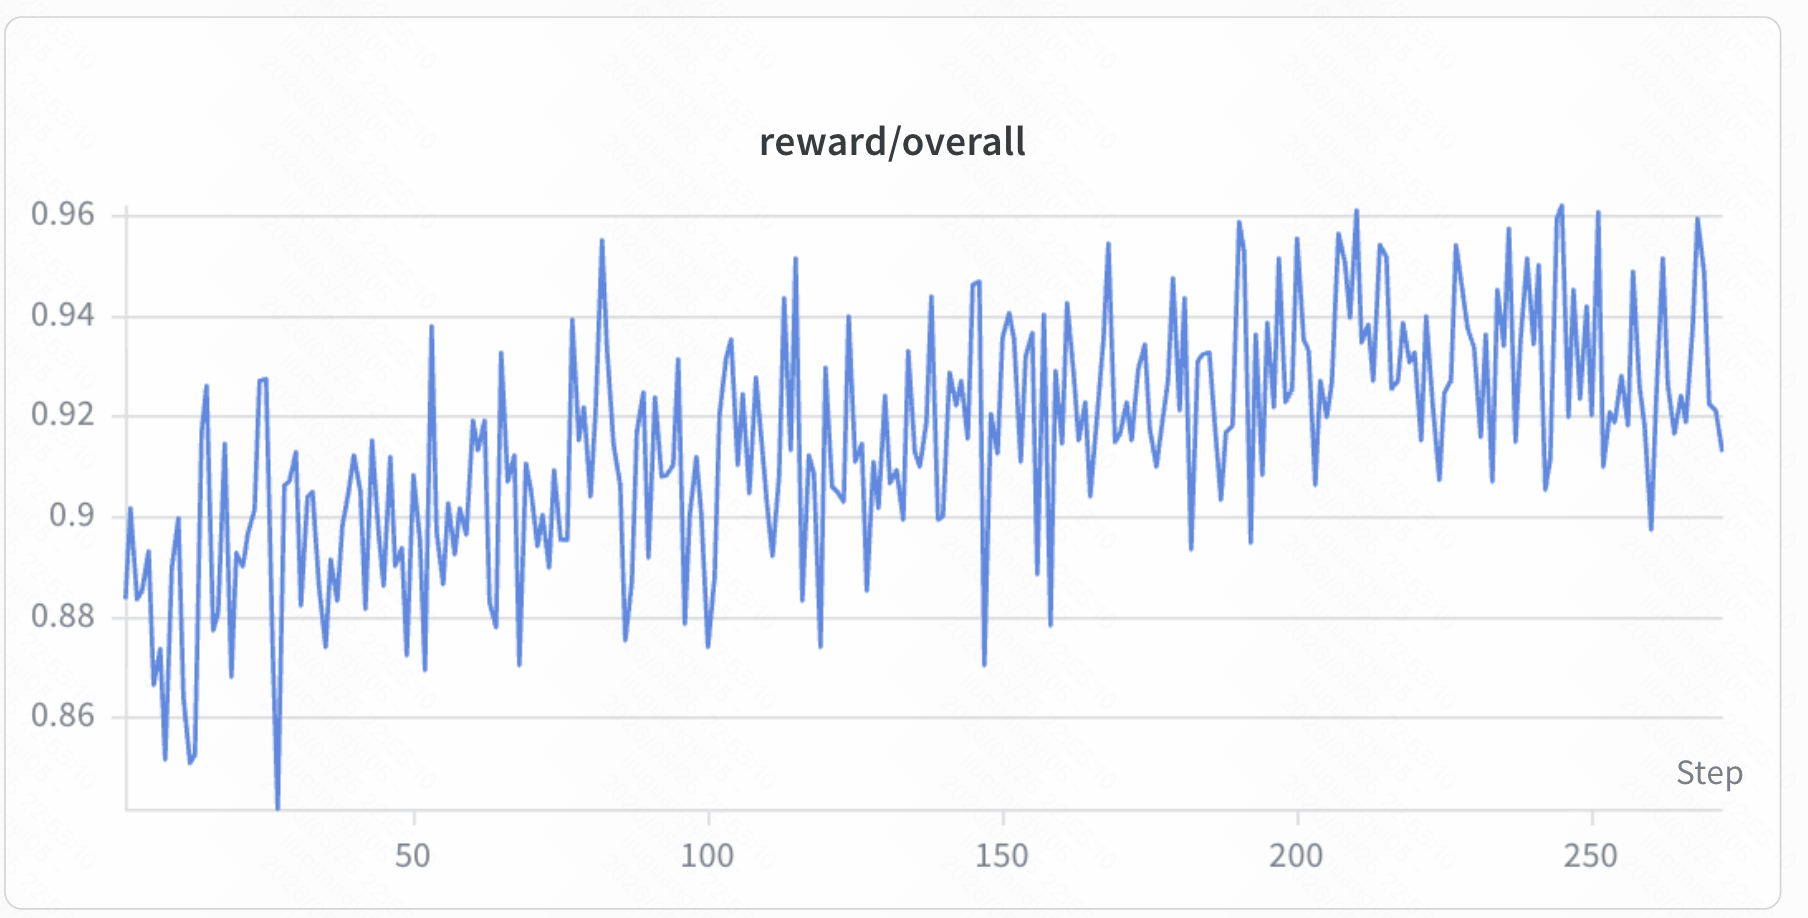
\includegraphics[width=\linewidth]{images/training-curves/qwen3vl-8b-training-900-tasks-reward-overall.png}
  \caption{\llmname{Qwen3-VL-8B}: overall}
\end{subfigure}
\hfill
\begin{subfigure}{0.32\textwidth}
  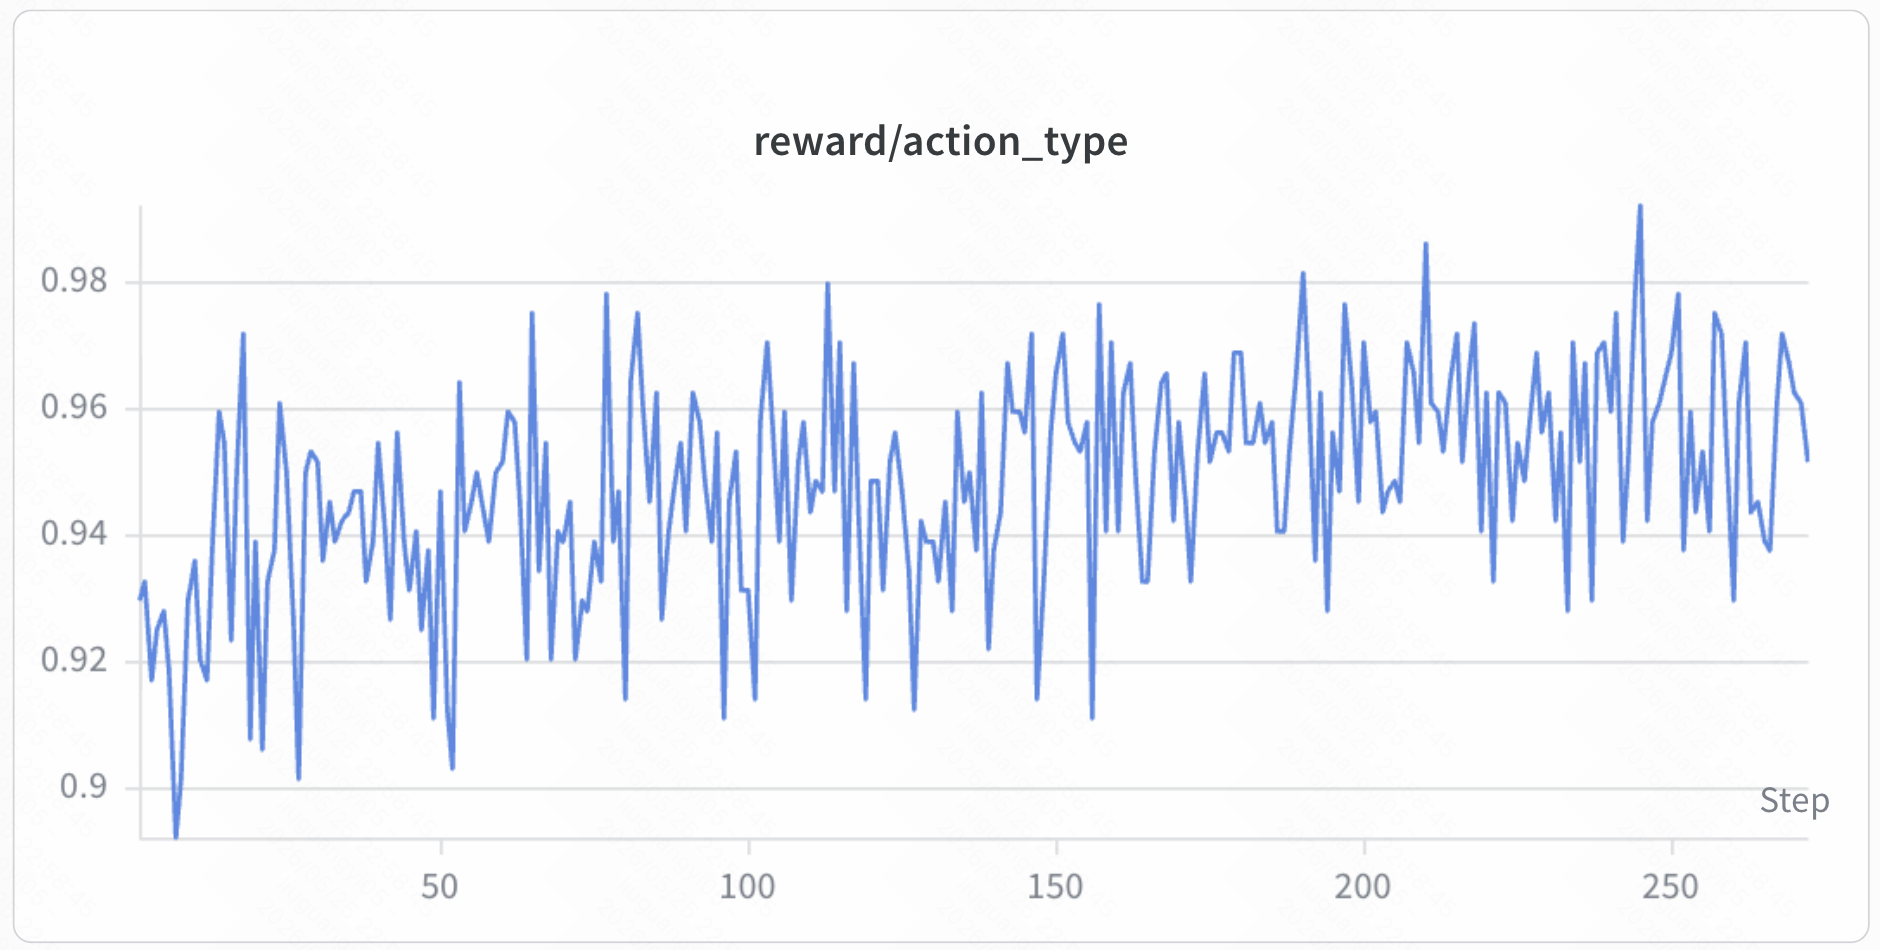
\includegraphics[width=\linewidth]{images/training-curves/qwen3-vl-8b-training-900-tasks-reward-action_type.png}
  \caption{\llmname{Qwen3-VL-8B}: action type}
\end{subfigure}
\hfill
\begin{subfigure}{0.32\textwidth}
  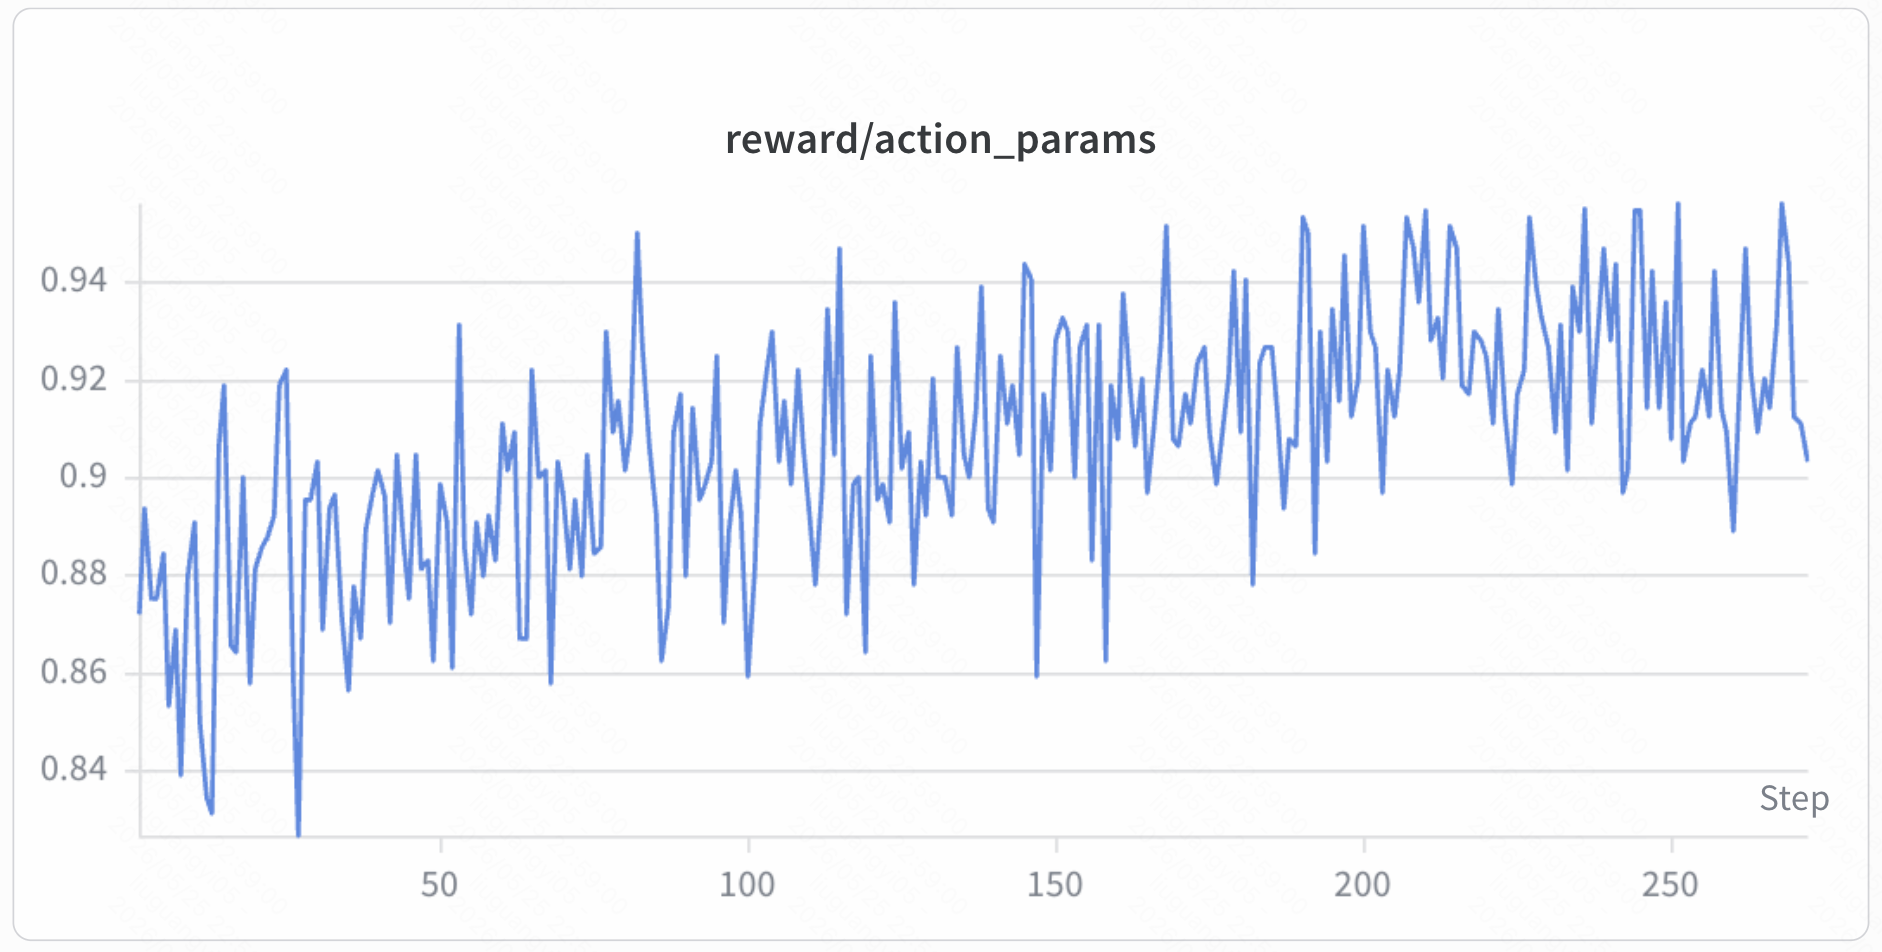
\includegraphics[width=\linewidth]{images/training-curves/qwen3-vl-8b-training-900-tasks-reward-action_params.png}
  \caption{\llmname{Qwen3-VL-8B}: arguments}
\end{subfigure}

\vspace{2mm}
\begin{subfigure}{0.32\textwidth}
  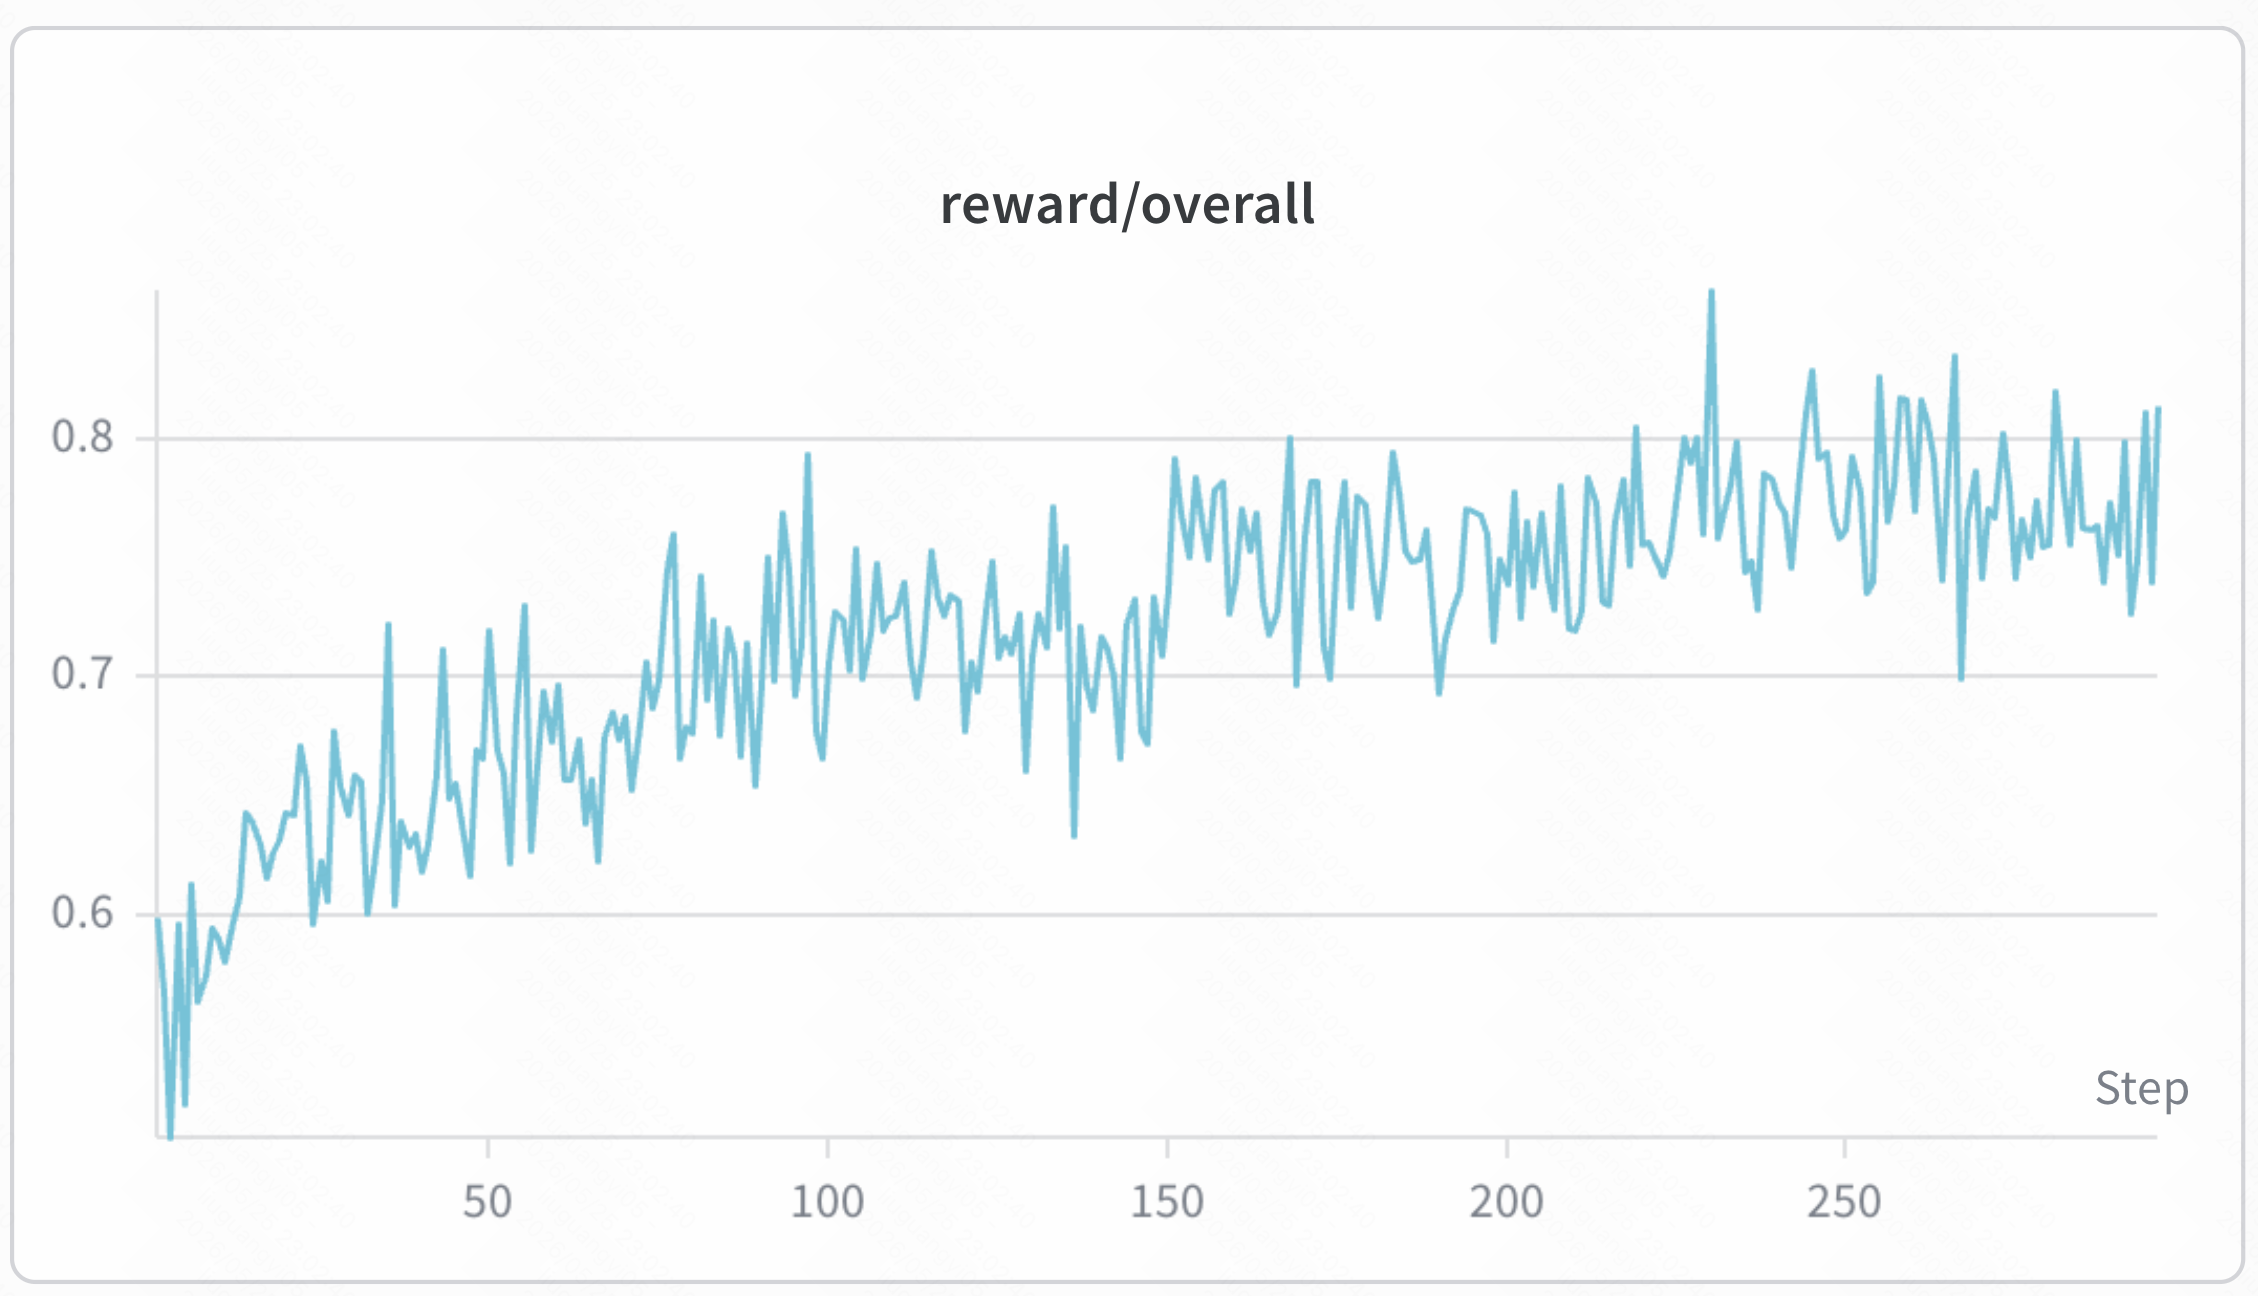
\includegraphics[width=\linewidth]{images/training-curves/gui-owl-1.5-8b-training-900-tasks-reward-overall.png}
  \caption{\llmname{GUI-Owl-1.5-8B}: overall}
\end{subfigure}
\hfill
\begin{subfigure}{0.32\textwidth}
  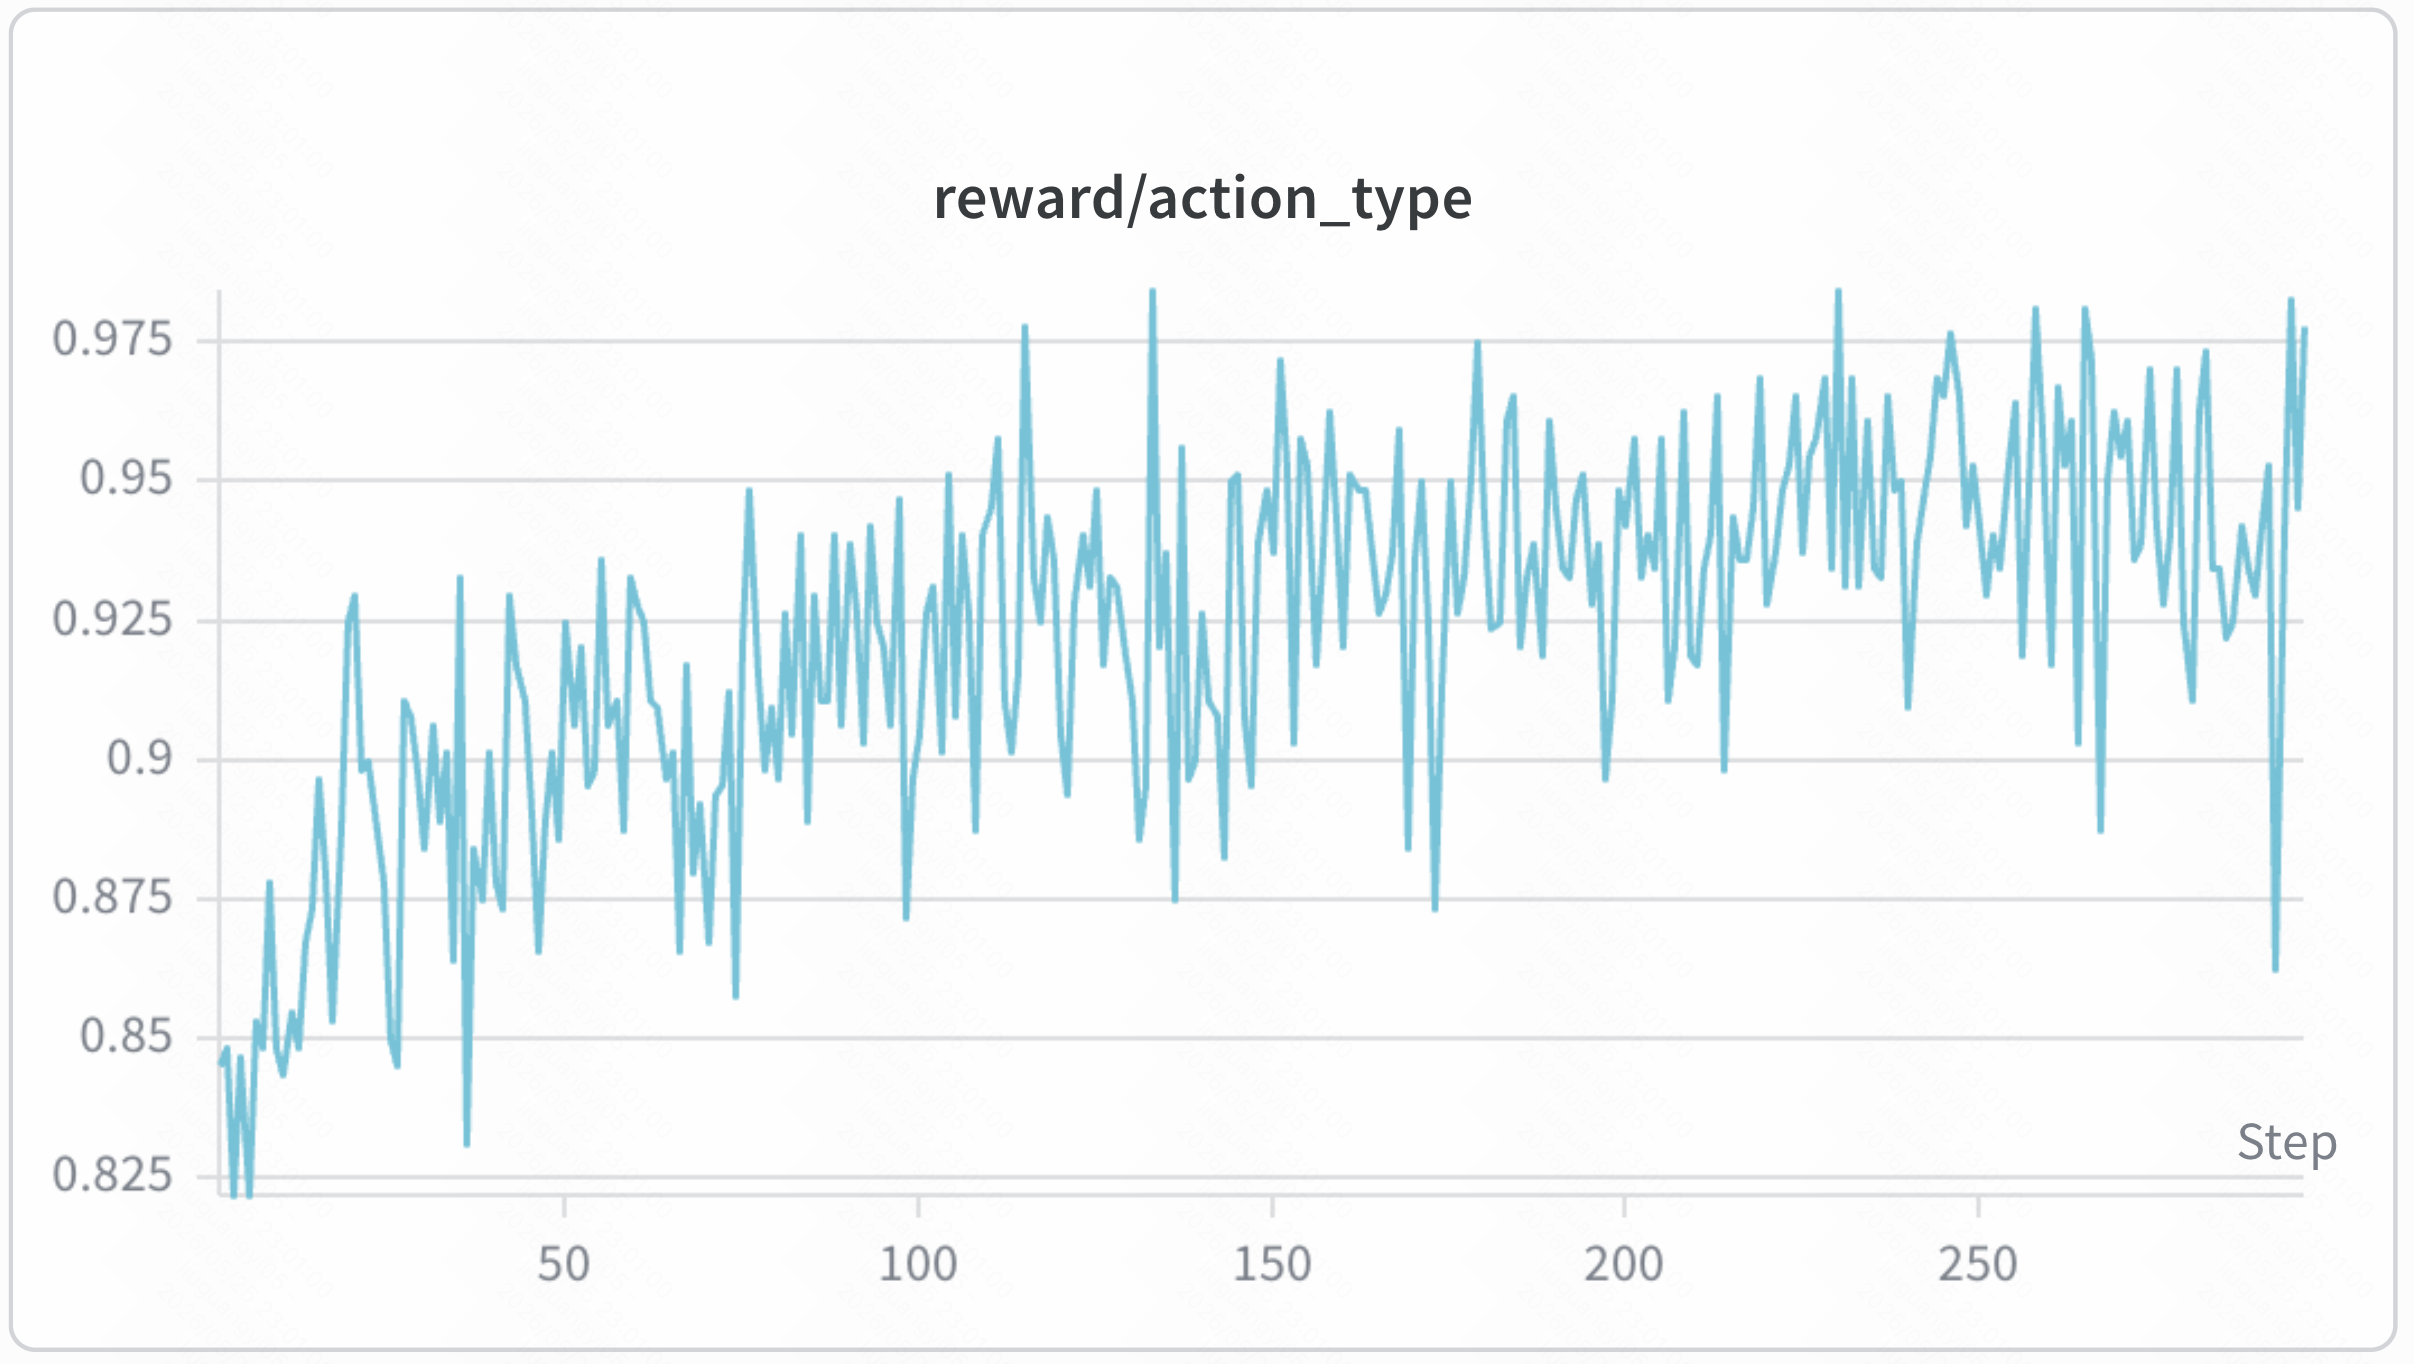
\includegraphics[width=\linewidth]{images/training-curves/gui-owl-1.5-8b-training-900-tasks-reward-action_type.png}
  \caption{\llmname{GUI-Owl-1.5-8B}: action type}
\end{subfigure}
\hfill
\begin{subfigure}{0.32\textwidth}
  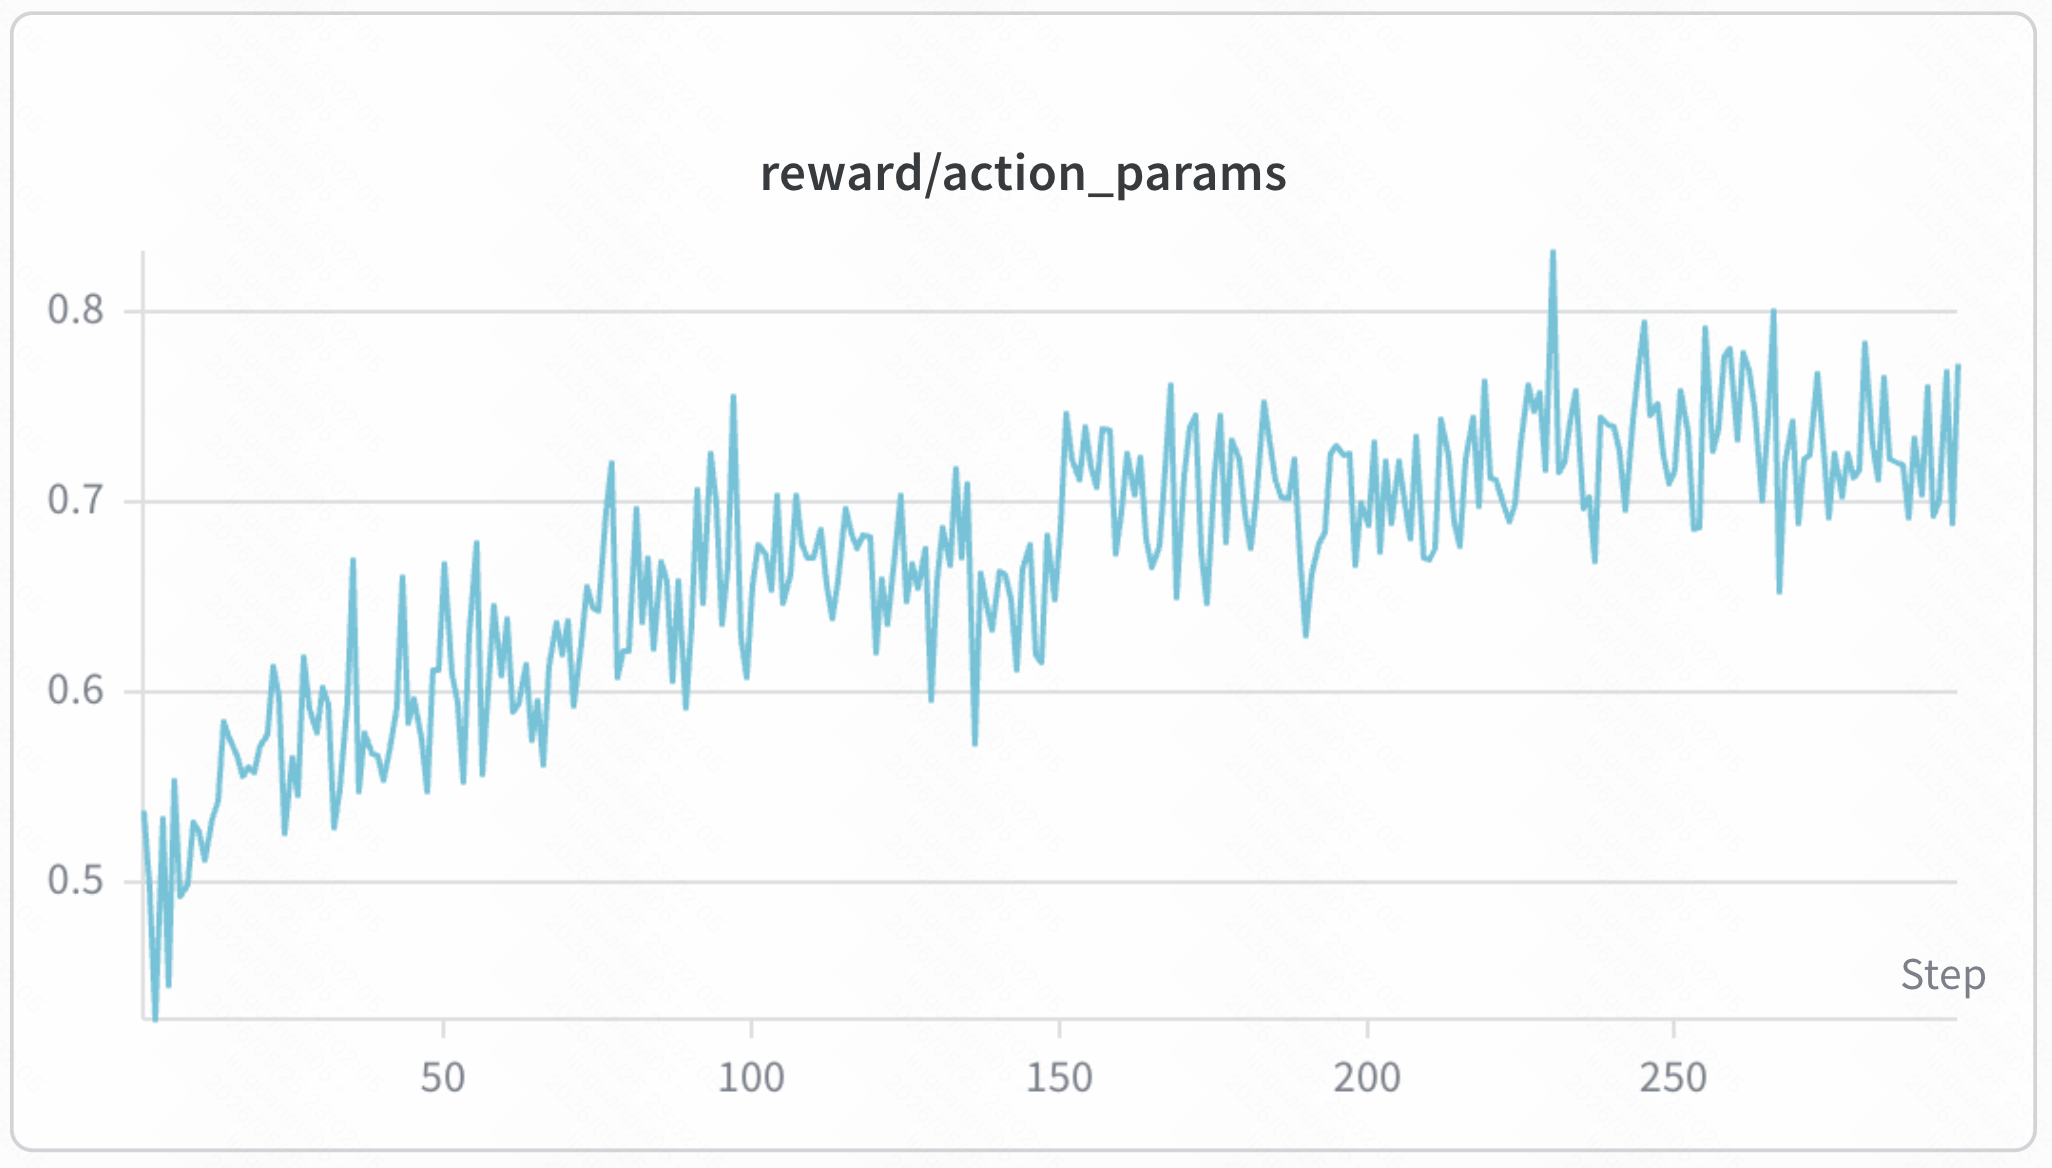
\includegraphics[width=\linewidth]{images/training-curves/gui-owl-1.5-8b-training-900-tasks-reward-action_params.png}
  \caption{\llmname{GUI-Owl-1.5-8B}: arguments}
\end{subfigure}
\caption{Training reward curves for the 900-task \hifpo runs. The overall reward combines action type and action arguments with weights 0.2 and 0.8.}
\label{fig:training_curves}
\end{figure*}

\paragraph{Track-completion cases.}
\label{sec:appendix_track_completion_cases}
Figures~\ref{fig:track_completion_androidworld_qwen}, \ref{fig:track_completion_mobileworld_qwen}, and~\ref{fig:track_completion_mobileworld_guiowl} provide paired base-versus-adapted trajectory comparisons on the same tasks. The examples complement the case study in Section~\ref{sec:case_study_error_analysis} by showing how adaptation changes full task-completion behavior across both AndroidWorld and MobileWorld.

\clearpage

\begin{figure*}[!p]
\centering
\begin{subfigure}[t]{0.49\textwidth}
  \centering
  \includegraphics[width=\linewidth,height=0.68\textheight,keepaspectratio]{images/track-completion-comparison/AndroidWorld-qwen-base.png}
  \caption{\llmname{Qwen3-VL-8B} base: failed}
\end{subfigure}
\hfill
\begin{subfigure}[t]{0.49\textwidth}
  \centering
  \includegraphics[width=\linewidth,height=0.68\textheight,keepaspectratio]{images/track-completion-comparison/AndroidWorld-qwen-rl.png}
  \caption{\llmname{ForgeQwen3-8B}: successful}
\end{subfigure}
\caption{\textbf{AndroidWorld track-completion comparison for \llmname{Qwen3-VL-8B}.}
On the same Broccoli recipe-deletion task, the base model falls into repeated scrolling after partial progress, while \ourmethod adaptation enables \llmname{ForgeQwen3-8B} to switch to a targeted search strategy and complete the remaining deletion.}
\label{fig:track_completion_androidworld_qwen}
\end{figure*}

\begin{figure*}[!p]
\centering
\begin{subfigure}[t]{0.49\textwidth}
  \centering
  \includegraphics[width=\linewidth,height=0.68\textheight,keepaspectratio]{images/track-completion-comparison/MobileWorld-qwen-base.png}
  \caption{\llmname{Qwen3-VL-8B} base: failed}
\end{subfigure}
\hfill
\begin{subfigure}[t]{0.49\textwidth}
  \centering
  \includegraphics[width=\linewidth,height=0.68\textheight,keepaspectratio]{images/track-completion-comparison/MobileWorld-qwen-rl.png}
  \caption{\llmname{ForgeQwen3-8B}: successful}
\end{subfigure}
\caption{\textbf{MobileWorld track-completion comparison for \llmname{Qwen3-VL-8B}.}
On the same multi-app academic-calendar and email task, the base model selects an underspecified semester result and then skips the calendar subtask, while \llmname{ForgeQwen3-8B} verifies the Spring 2026 deadline window, creates the calendar event, and proceeds to the email workflow.}
\label{fig:track_completion_mobileworld_qwen}
\end{figure*}

\begin{figure*}[!p]
\centering
\begin{subfigure}[t]{0.49\textwidth}
  \centering
  \includegraphics[width=\linewidth,height=0.68\textheight,keepaspectratio]{images/track-completion-comparison/MobileWorld-guiowl-base.png}
  \caption{\llmname{GUI-Owl-1.5-8B} base: failed}
\end{subfigure}
\hfill
\begin{subfigure}[t]{0.49\textwidth}
  \centering
  \includegraphics[width=\linewidth,height=0.68\textheight,keepaspectratio]{images/track-completion-comparison/MobileWorld-guiowl-rl.png}
  \caption{\llmname{ForgeOwl-8B}: successful}
\end{subfigure}
\caption{\textbf{MobileWorld track-completion comparison for \llmname{GUI-Owl-1.5-8B}.}
On the same invoice recalculation and email task, the base model leaves the invoice context too early and sends an incorrect amount, while \llmname{ForgeOwl-8B} preserves the key invoice conditions, shares the document into Mail, and sends the correct recalculated total.}
\label{fig:track_completion_mobileworld_guiowl}
\end{figure*}

